\documentclass[11pt,a4paper]{article}
\usepackage[margin=0.78in]{geometry}
\usepackage{graphicx}
\usepackage{booktabs}
\usepackage{url}
\usepackage{float}
\usepackage{caption}
\usepackage{amsmath}

\title{Learning-Augmented Disk Scheduling Under Changing Workload Patterns}
\author{CSE307 Operating Systems Term Paper}
\date{October 2026}

\begin{document}
\maketitle

\begin{abstract}
Disk scheduling policies can behave very differently when request locality and ordering change. This project compares FCFS, SSTF, SCAN, and C-SCAN in a controlled simulation and adds a lightweight learned selector based on \texttt{DecisionTreeClassifier}. Each workload window is converted into simple numerical features, labelled by the scheduler with the lowest simulated head movement, and evaluated on separate synthetic windows. On the generated test split the decision tree reached 84.38\% accuracy. SSTF was strongest for localized, uniform, and bursty windows, while FCFS was competitive on upward directional windows. The learned selector usually stayed close to the oracle, but it also made visible mistakes when directional windows resembled the SSTF-dominated training patterns.
\end{abstract}

\section{Introduction}
Disk scheduling is usually introduced through fixed policies such as FCFS, SSTF, SCAN, and C-SCAN. These algorithms are useful because their behavior is understandable, but they are also sensitive to request order and locality. A request trace that is nearly sequential can make FCFS look good, while a random or clustered trace often rewards a policy that moves toward nearby cylinders. Operating systems texts discuss these policies as part of storage management and I/O scheduling because head movement is a major cost in the simplified mechanical disk model \cite{silberschatz2018osc,arpacidusseau2018ostep}.

This project asks whether a small learned component can choose among classical schedulers when the workload pattern changes. The aim is not to build a production I/O scheduler or measure real disk latency. The experiment is a simulation where total head movement in cylinders is used as a seek-distance proxy. That simplification keeps the project explainable while still showing why one fixed policy may be a poor choice for every workload.

\section{Methodology}
\subsection{Classical Disk Scheduling Algorithms}
FCFS services requests exactly in arrival order. SSTF repeatedly chooses the pending request closest to the current head position; if two requests are equally close, this implementation chooses the lower cylinder first. SCAN is implemented as true elevator SCAN, not LOOK: with upward direction it services requests above the head, moves to cylinder 199, then reverses. C-SCAN is also true circular SCAN: after reaching cylinder 199 it wraps to cylinder 0 and the wrap distance is counted. Requests at the current head are serviced first with zero movement.

\subsection{Synthetic Workloads}
All experiments use cylinders 0 through 199, initial head position 50, upward SCAN/C-SCAN direction, and 40 requests per window. Four workload families are generated with deterministic seeds: uniform windows spread requests across the disk; localized windows draw from one narrow region; directional windows move mostly upward with small jitter; bursty windows use three locality regions in sequence. This design is related to the general idea that programs and systems often show locality that can move over time \cite{denning1968working}.

The workload-shift experiment uses 24 windows. The first 12 are directional and the next 12 are uniform. The selector predicts once per window, so it can change its decision after the phase boundary.

\subsection{Learning-Augmented Selector}
For each training window, the same request list is passed to FCFS, SSTF, SCAN, and C-SCAN. The label is the scheduler with the lowest total head movement, using FCFS, SSTF, SCAN, then C-SCAN as the deterministic tie order. The features are request mean, standard deviation, range, minimum, maximum, mean and median consecutive movement, increasing and decreasing transition ratios, direction-change ratio, and distance from the current head to the request mean. Scheduler performance is not included as a feature, which avoids target leakage.

The classifier is a scikit-learn decision tree \cite{sklearnDecisionTree} with \texttt{max\_depth=4}, \texttt{min\_samples\_leaf=8}, and \texttt{random\_state=307}. The dataset contains 640 generated windows, split into 480 training windows and 160 test windows. Label counts were FCFS: 93, SSTF: 535, SCAN: 12, C-SCAN: 0. The trained tree had depth 4 and 11 leaves.

\subsection{Experimental Setup}
The main evaluation uses 50 fresh windows per workload type, separate from the training seeds. Each row records the fixed scheduler movements, the predicted scheduler, the actual best scheduler, the learned-selector movement, and the oracle-best movement. The oracle is not available to the classifier before prediction; it is only used for evaluation.

\section{Results}
\begin{figure}[H]
  \centering
  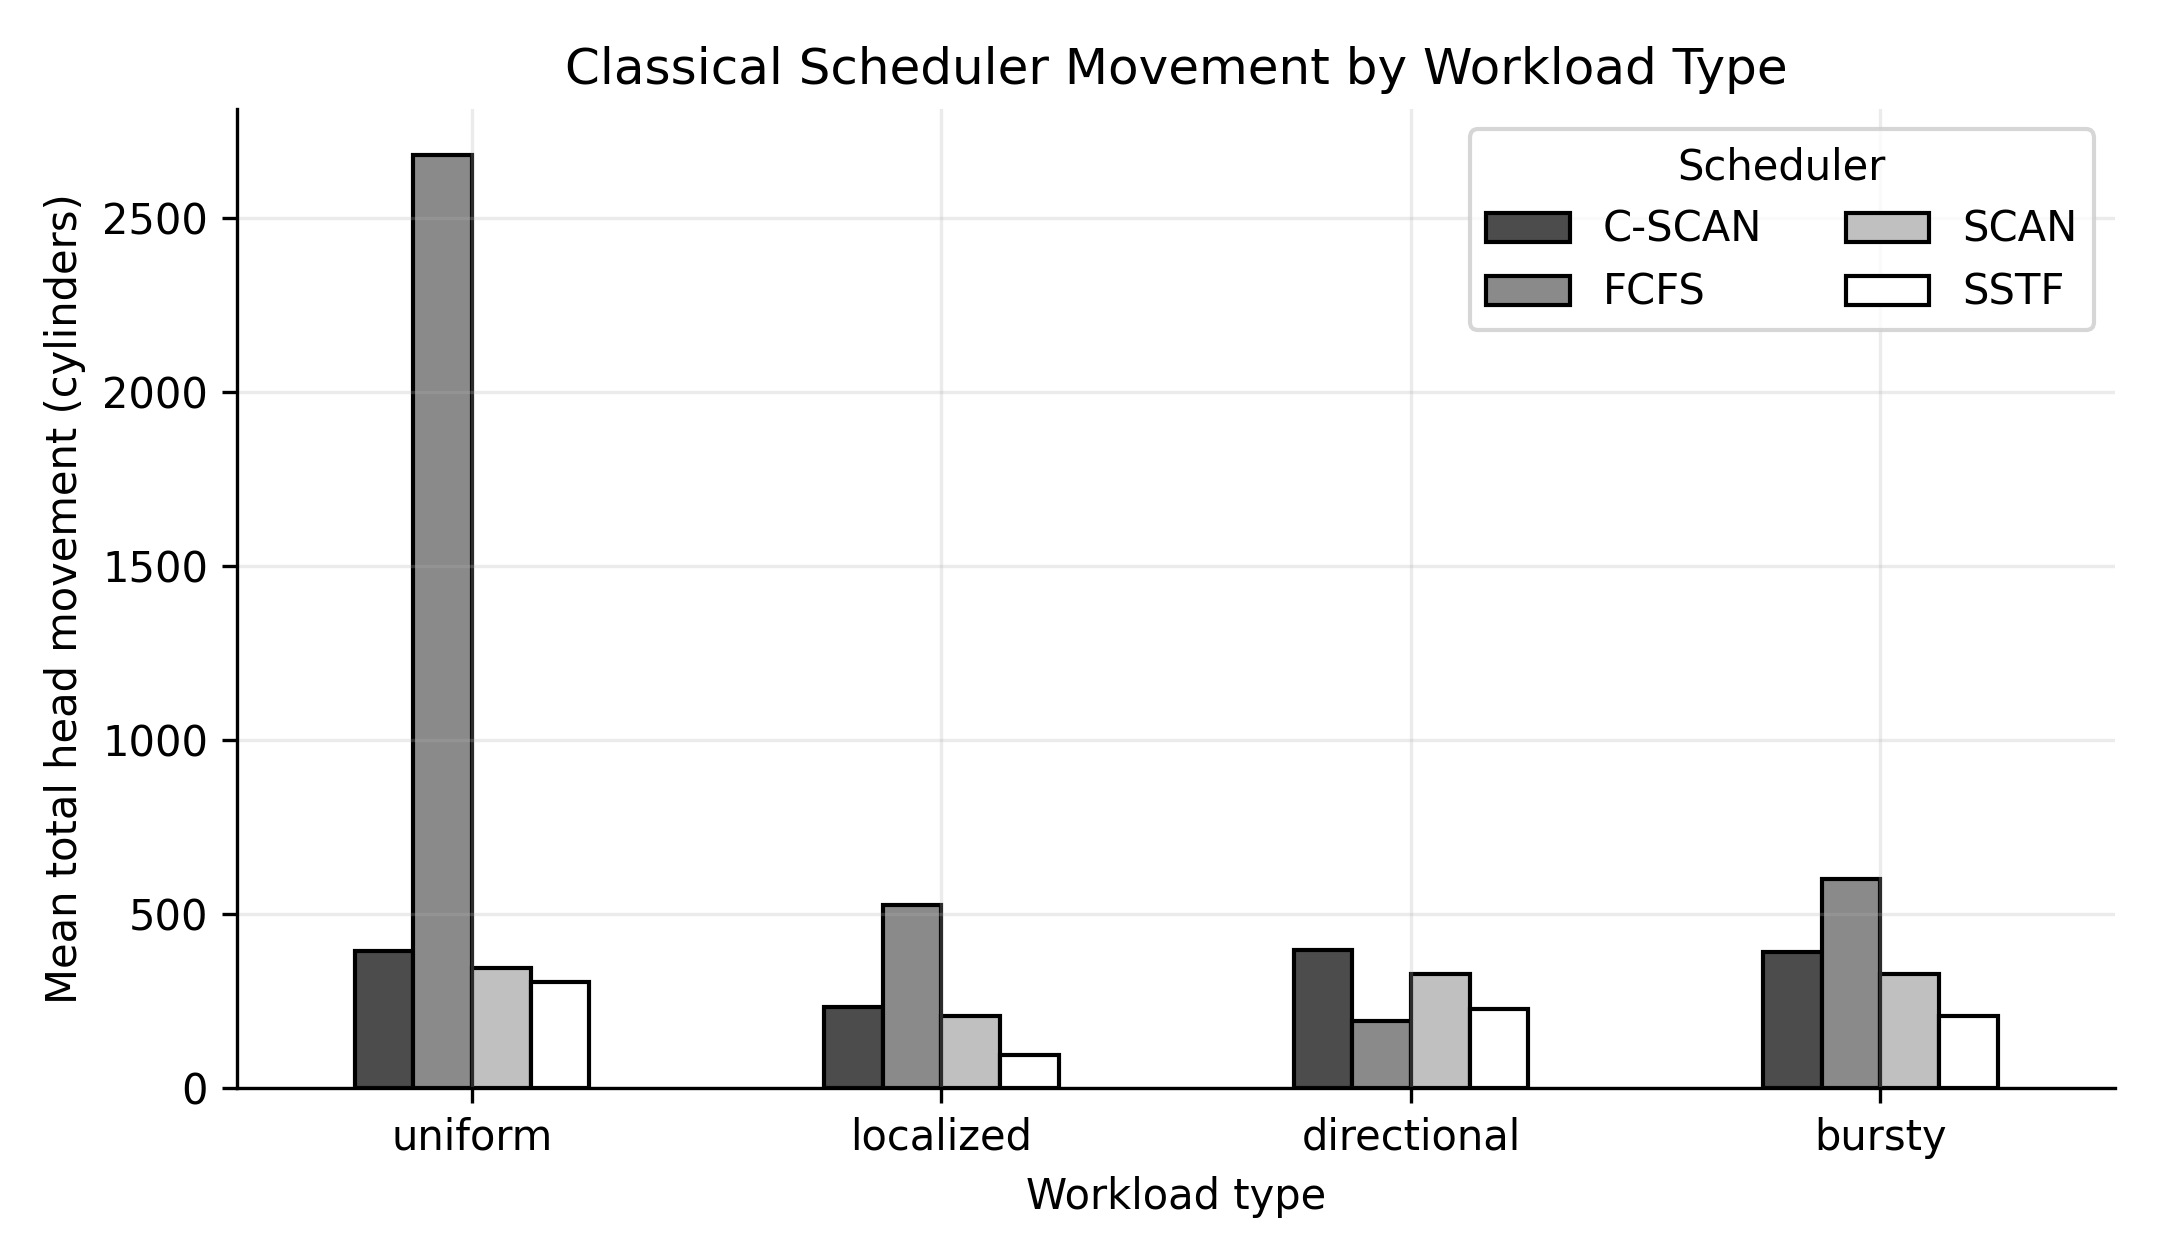
\includegraphics[width=0.92\linewidth]{../figures/classical_scheduler_comparison.png}
  \caption{Mean simulated total head movement for the four classical schedulers across 50 windows per workload type.}
  \label{fig:classical}
\end{figure}

Figure~\ref{fig:classical} shows that FCFS is very sensitive to request order. For uniform windows, FCFS averaged 2680.20 cylinders of movement, while SSTF averaged 303.26. Localized windows also favored SSTF, which averaged 93.32 cylinders compared with 524.24 for FCFS. Directional windows were different: FCFS averaged 192.22 cylinders and was close to the oracle because the requests already followed a mostly upward order.

\begin{figure}[H]
  \centering
  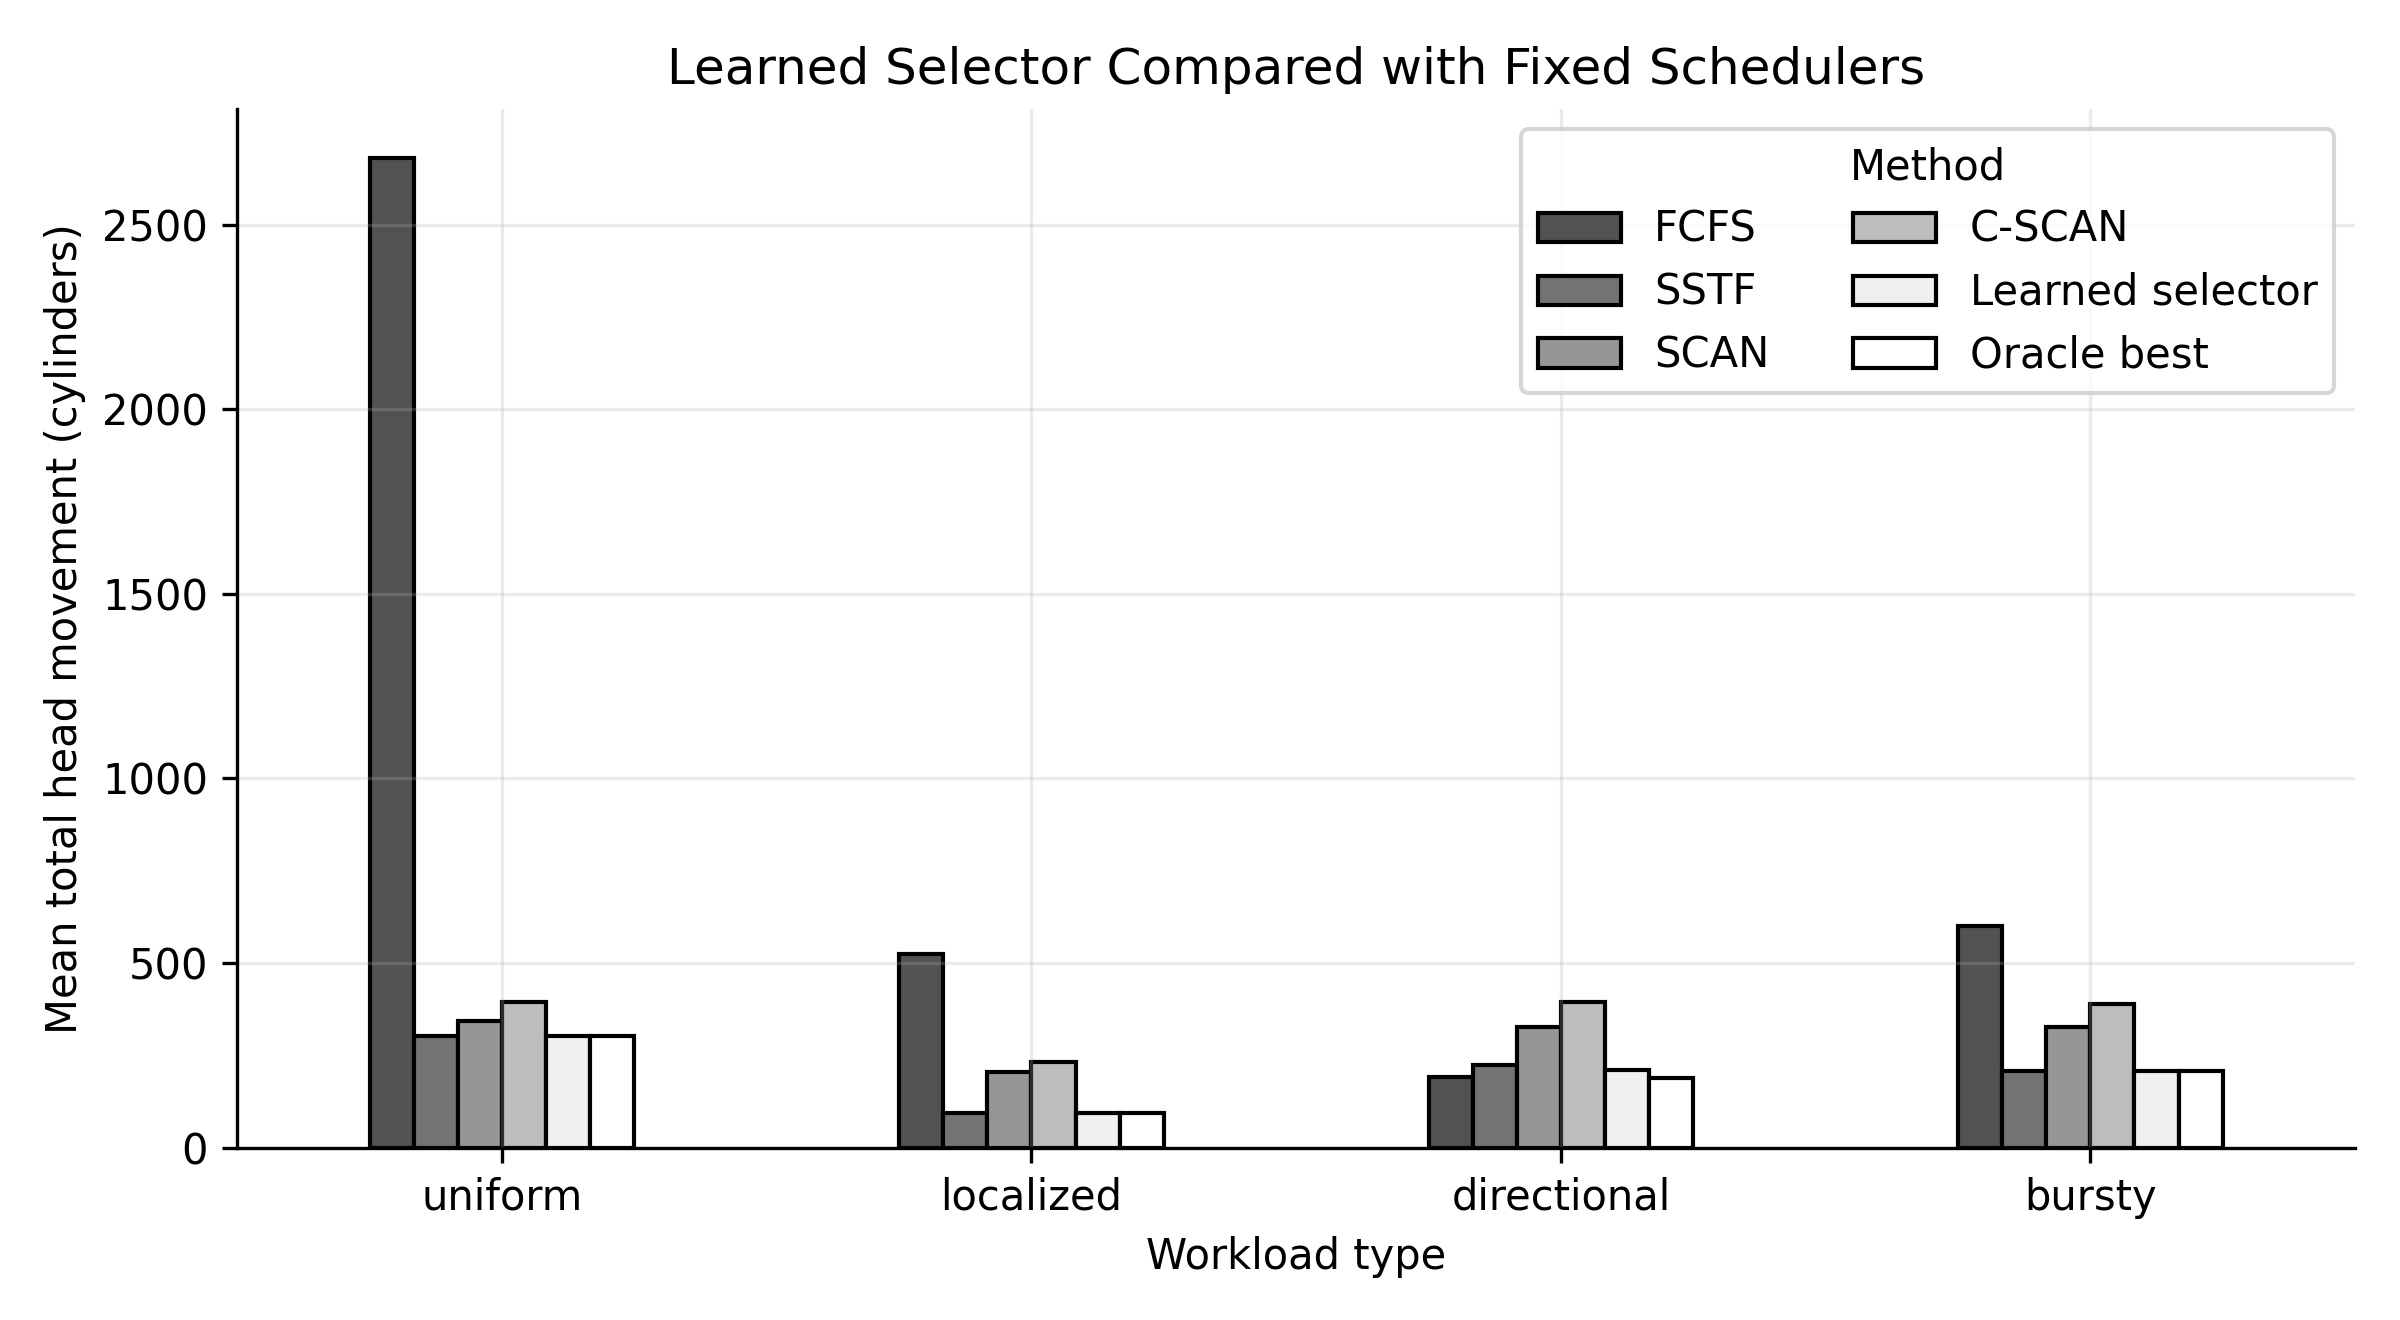
\includegraphics[width=0.92\linewidth]{../figures/learned_selector_comparison.png}
  \caption{Learned selector compared with fixed schedulers and the oracle best scheduler.}
  \label{fig:selector}
\end{figure}

The learned selector tracked SSTF closely on localized, uniform, and bursty workloads. For bursty windows it averaged 206.86 cylinders, almost identical to the oracle average of 206.80. On localized windows it exactly matched the oracle mean because SSTF dominated those labels. Directional windows were harder: the learned selector averaged 211.16 cylinders while the oracle averaged 187.98. This gap came from some FCFS-favorable directional windows being predicted as SSTF.

\begin{table}[H]
\centering
\caption{Decision tree and workload-shift results generated from CSV files.}
\label{tab:model}
\begin{tabular}{lr}
\toprule
Measurement & Value \\
\midrule
Decision tree test accuracy & 84.38\% \\
Training windows & 480 \\
Test windows & 160 \\
Tree depth & 4 \\
Tree leaves & 11 \\
Directional phase learned mean & 214.50 cylinders \\
Directional phase oracle mean & 193.25 cylinders \\
Directional phase prediction accuracy & 41.67\% \\
Uniform phase learned mean & 287.58 cylinders \\
Uniform phase oracle mean & 286.08 cylinders \\
Uniform phase prediction accuracy & 91.67\% \\
\bottomrule
\end{tabular}
\end{table}

\begin{figure}[H]
  \centering
  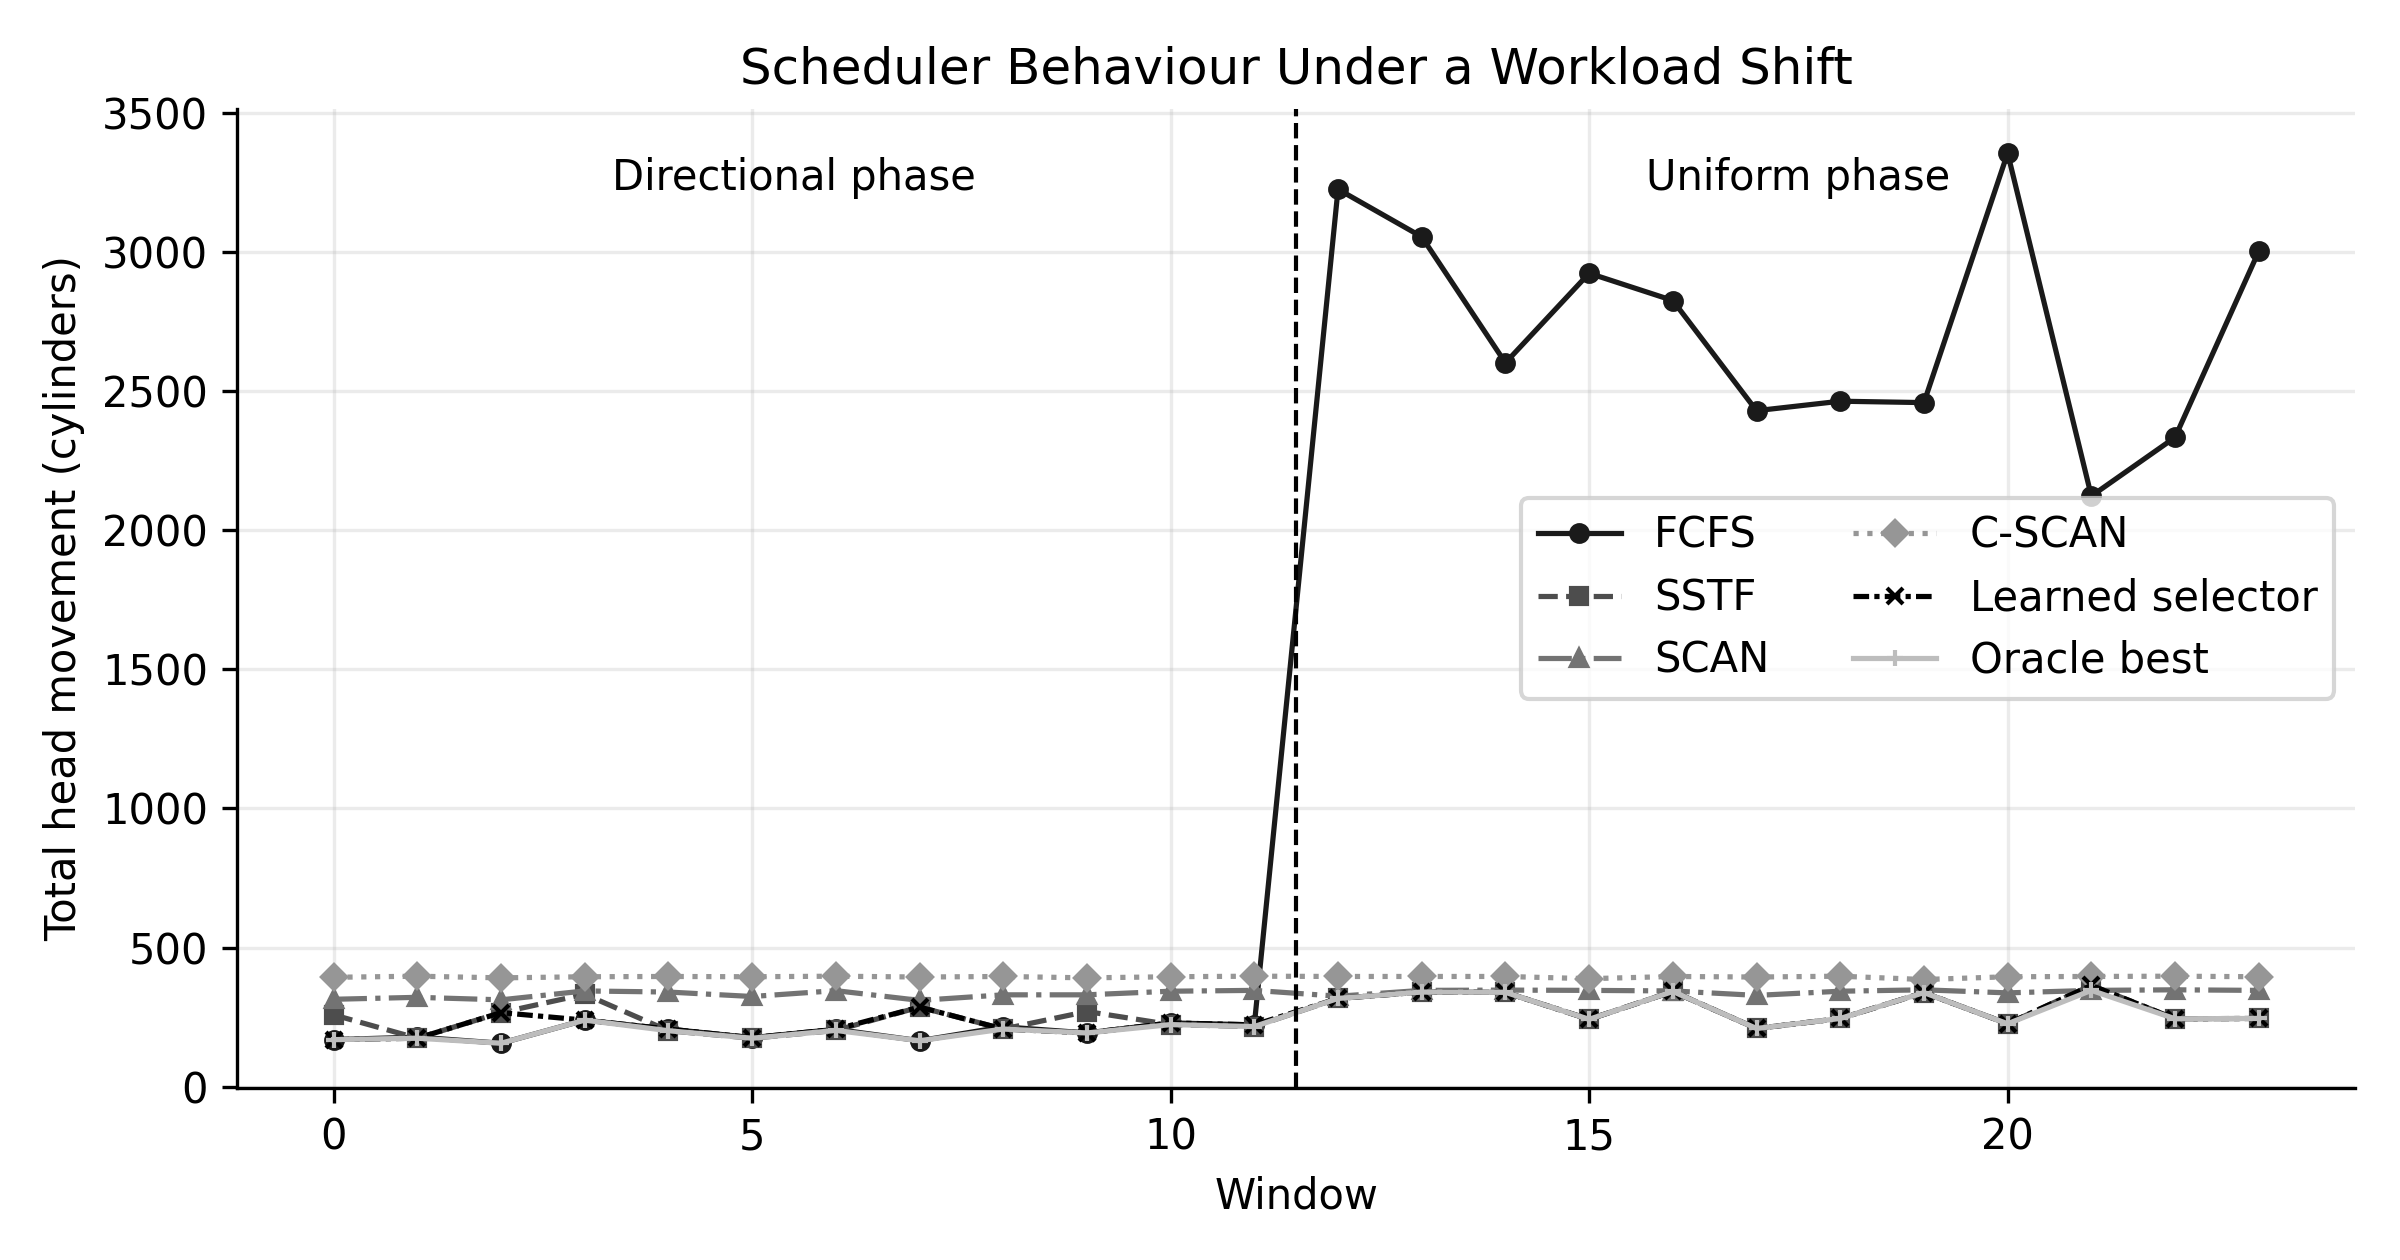
\includegraphics[width=0.92\linewidth]{../figures/workload_shift_behavior.png}
  \caption{Per-window behavior when the workload changes from directional to uniform requests.}
  \label{fig:shift}
\end{figure}

The workload-shift run in Figure~\ref{fig:shift} shows that the selector did not make one prediction for the whole trace. It predicted FCFS for several directional windows and SSTF for all uniform windows. The transition is visible at the phase boundary, but the directional phase also shows the selector's main weakness: it sometimes chose SSTF when FCFS or SCAN was slightly better.

\section{Discussion}
The results follow the expected behavior of the algorithms. FCFS has no spatial awareness, so random uniform requests create long jumps across the disk. SSTF directly minimizes the next local movement and therefore performs well on clustered, bursty, and many uniform windows. SCAN and C-SCAN are less competitive in this finite-window experiment because their endpoint conventions are real SCAN and C-SCAN, so they pay for movement to cylinder 199 and, for C-SCAN, the wrap to cylinder 0. This is technically correct but makes C-SCAN unattractive under the simple total-movement metric.

The decision tree learned mostly from locality and ordering features. The most important feature in the final model was mean absolute consecutive movement, which separates nearly sequential windows from random jumps. The model's 84.38\% test accuracy is not perfect, and that is useful rather than embarrassing. The labels are imbalanced because SSTF genuinely wins most generated windows. C-SCAN received no training labels because its counted wrap-around never produced the minimum movement in this setup. A larger or different disk model could change that, but this experiment reports the generated results rather than forcing all classes to appear.

Several limitations matter. The simulation ignores rotational latency, queue arrival times, request deadlines, caching, real device firmware, and kernel overhead. Total head movement is only a proxy for seek cost. The learned selector also depends on the synthetic training distribution; if real traces differ, the decision tree could make worse choices. Still, the experiment shows a reasonable OS idea at undergraduate scale: simple workload features can help choose among classical policies, but the learned layer should be treated as a helper, not as evidence that classical schedulers are obsolete.

\section{Conclusion}
This project implemented and tested FCFS, SSTF, SCAN, and C-SCAN, generated reproducible workload windows, labelled each window using actual scheduler performance, and trained a lightweight decision-tree selector. The selector reached 84.38\% test accuracy and stayed close to the oracle on localized, uniform, and bursty workloads. Directional windows exposed the main trade-off: the learned selector can adapt between phases, but incorrect predictions can still lose to a well-matched fixed scheduler. The result supports a cautious learning-augmented approach where classical algorithms remain the execution mechanisms and machine learning only selects among them.

\bibliographystyle{IEEEtran}
\bibliography{references}

\end{document}
